Una partícula se desplaza a lo largo de una recta. Su posición, $d$, en relación con un punto $O$ de la recta, varía en el tiempo de acuerdo con el gráfico de la figura de este problema. Considerando los instantes $t_A$, $t_B$, $t_C$ y $t_D$:
\begin{enumerate}
    \item ¿Para cuál de ellos, la partícula se halla más cercana a $O$? ¿Y más lejos?
    \item Coloque en orden creciente los valores de la velocidad de la partícula en dichos instantes.
\end{enumerate}
\begin{figure}[h!]
  \centering
  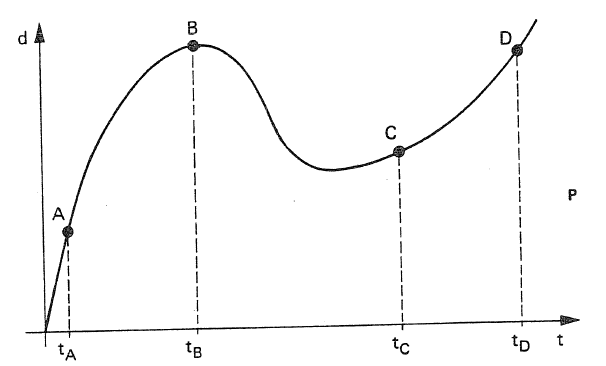
\includegraphics[scale=0.5]{figuras/fig_alvarenga_p91_26.png}
  \caption{Problema 2}
\end{figure}
